\documentclass[10pt,a4paper]{scrartcl}
\usepackage[utf8]{inputenc}
\usepackage[T1]{fontenc}
\usepackage[french]{babel}
\usepackage{textcomp}
\usepackage{lmodern}
\usepackage{graphicx}
\usepackage[dvipsnames,svgnames]{xcolor}
\usepackage{microtype}
\usepackage{hyperref} \hypersetup{colorlinks=true,linkcolor=Brown,urlcolor=Navy,
breaklinks=true,pdfstartview=XYZ}
\title{Rapport BD Librairie}
\author{Jeanne BARASTIER, Yann ROBLIN, Tom BARTIER}
\begin{document}
\maketitle
\begin{abstract}
    Dans le cadre du cours de remise à niveau de la première année de master nous devons réaliser une base de données en groupe. Le but est d’introduire, et de familiariser 
    les personnes ne venant pas de la licence informatique aux bases de la conception d’une base de données, 
    aux commandes et langage SQL et à la création d’une application simple via le langage de programmation python. 
    Le projet se sépare en deux étapes distinctes. La première étape consiste à concevoir et construire une base de 
    données de notre choix. La deuxième étape consiste à réaliser une application qui exploitera cette base de données.
\end{abstract}

\tableofcontents

\newpage
\section{Consignes}
Le travail qui nous est demandé n’est pas uniquement la création d’une base de 
données mais bel et bien la réalisation d’un petit projet. C’est pour cela qu’en 
plus d’une série de tables nous devons réaliser une série de tâches. Tout d’abord nous 
devons choisir un contexte pour notre base de données. Après en avoir choisi un, il faut
 créer un cahier des charges afin de définir nos objectifs. Ensuite vient la conception
  du Modèle Entité Association (MEA) de notre base de données. Une fois les étapes 
  précédentes réalisées nous pouvons passer à la partie SQL du projet. Tout d’abord il 
  y a la création des tables décrites dans le MEA. Une fois créées, nous devons remplir
   les tables à l’aide de requêtes. En plus des tables nous devons ajouter au moins deux
    déclencheurs. Une fois la base créée nous écrirons une série pertinente 
    d’instructions afin de la valider ainsi que deux exemples de cas d’utilisations 
    concurrentes qui poseraient problème. Tout ceci est à terminer pour fin septembre. 
Une application exploitant la base de données doit être présentée fin octobre.

\section{Librairie}
Le projet qu’on a choisi est la création d’une application à destination du personnel d’une librairie non initié au SQL. Elle doit principalement permettre de mettre à jour 
et consulter les stocks, les achats et les emprunts de livres. Nous avons fait ce choix car il s’agit d’un exemple simple et 
longuement traité pendant la licence. Comme il s’agit d’un projet d’initiation, la base de données sera assez simple et ne comportera donc que les éléments que nous jugeons essentiels.

\section{Cahier des charges}

\begin{itemize}
    \item L’application sera destinée au personnel d’une librairie non initié à SQL.
    \item Il faut que l'application soit ergonomique, simple d'utilisation tout en restant fonctionnelle.
    \item Elle permet de consulter les différentes tables de la base de données via des actions simples par un non initié à SQL.
    \item Elle doit permettre au personnel de modifier les différentes tables de la base de données via des actions simples pour un non initié à SQL.
    \item Chaque action réalisée sur l'application notamment concernant la modification des tables doit avoir un retour visuel.
\end{itemize}

\section{La base de données}

\begin{figure}
    \centering
    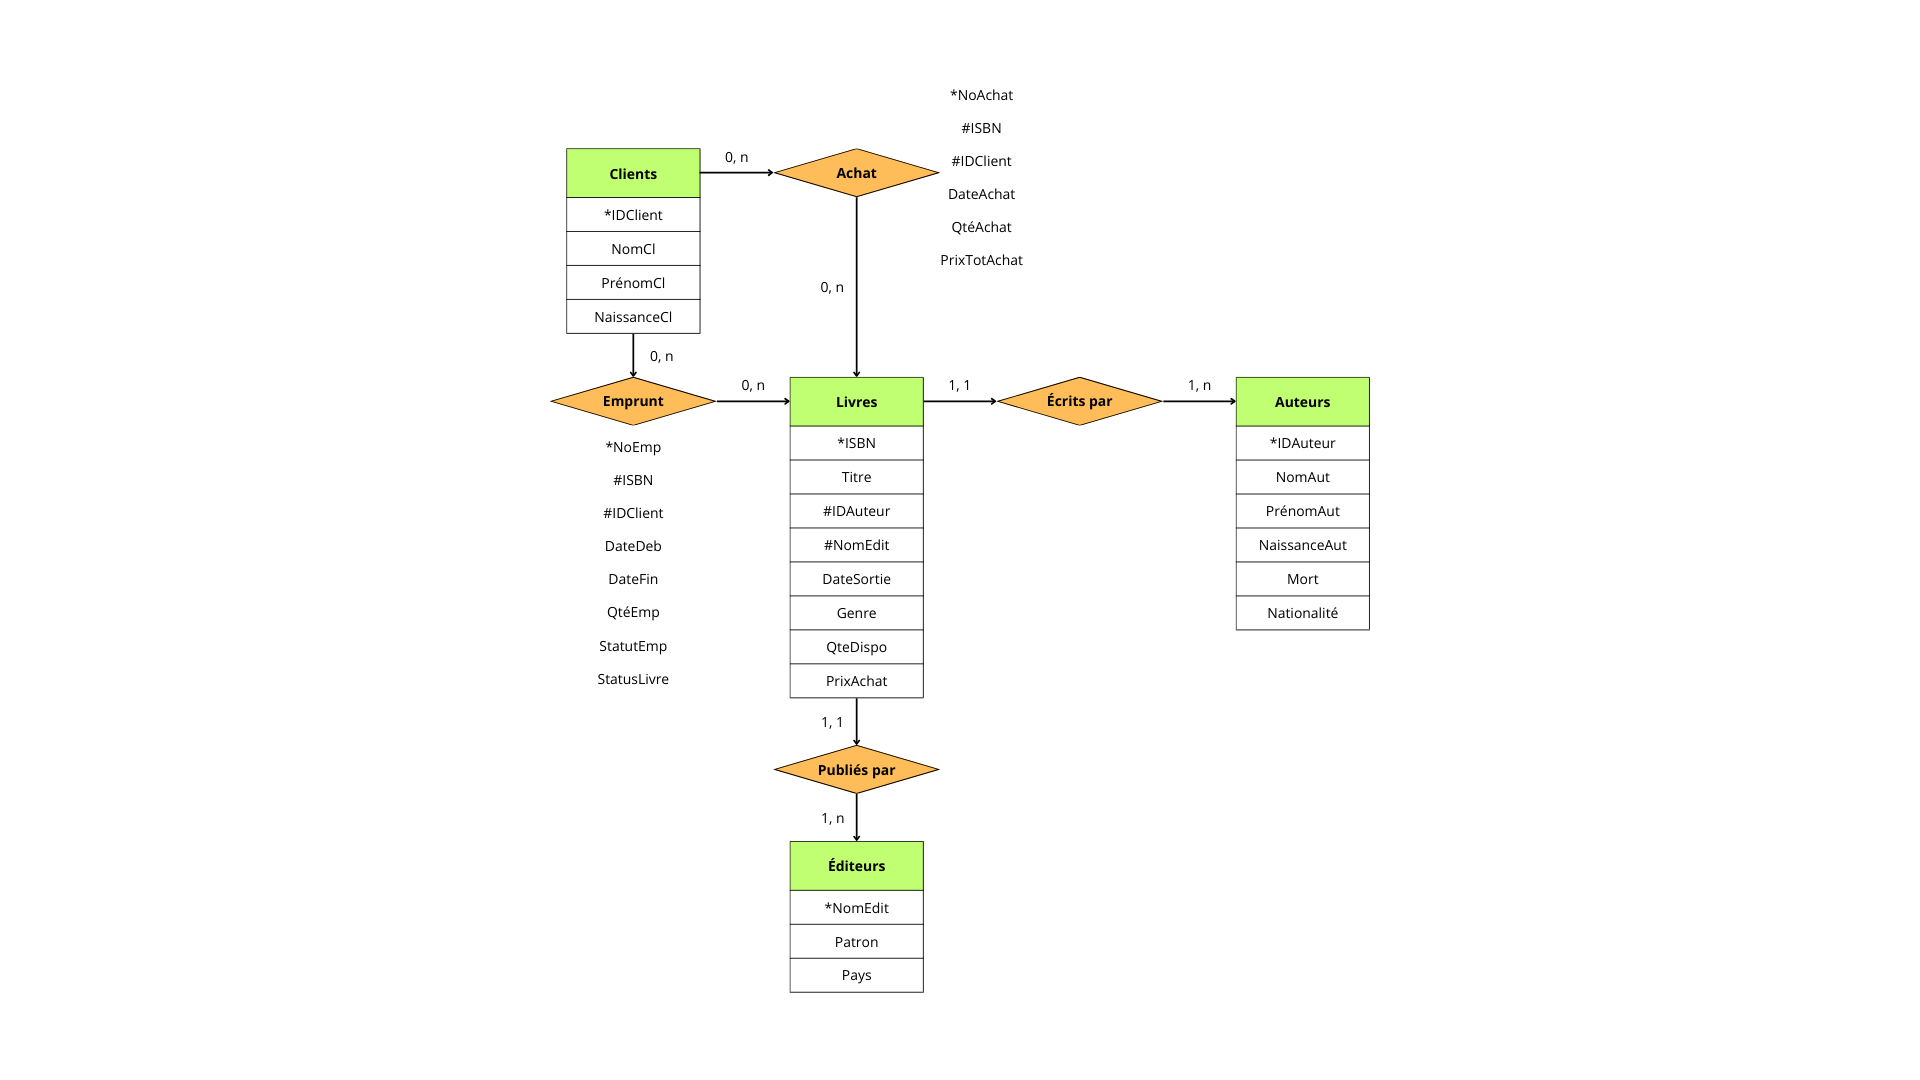
\includegraphics[trim=5cm 0cm 5cm 0cm, clip, width=1.2\textwidth]{MEA_BD}
    \caption{Modèle Entité Association}\label{fig.mea}
\end{figure}



\begin{itemize}
    \item Une table « Auteurs » qui contient les informations de chaque auteur des livres proposés à la vente ou à l’emprunt. Chaque auteur est différencié par un identifiant unique de 
    type entier. Un auteur possède un nom, un prénom, une date de naissance, la date de sa mort qui est vide si l’auteur est en vie, et une nationalité.
\end{itemize}

\end{document}